To identify the effectiveness of national cybersecurity policies,
it is essential to analyze the correlation between the implementation of these policies and the subsequent trends in cybercrime.
By examining the distribution of cybercrimes and comparing it with the timing and content of various national policies,
we can discern patterns that highlight which measures are particularly effective or ineffective.
This analysis will focus on key metrics such as the reduction in
cybercrime incidents, the success rate of prosecutions, and the overall resilience of national cybersecurity infrastructures.
Through this data-driven approach,
we aim to provide actionable insights for the development and refinement of cybersecurity policies.
\subsection{Selection of Representative Centroid Countries}\label{subsec:selection-of-representative centroid-countries} %4.1
Having constructed a clustering model to categorize countries into five clusters (T1 to T5) based on GCI and other relevant metrics,
we now proceed to analyze the effectiveness of cybersecurity policies within each cluster.
To ensure a representative and data-driven analysis,
we will select one central country from each cluster that meets the following criteria:
\begin{itemize}
    \item \textbf{Representativeness:}
    The selected country should typify the overall characteristics of its cluster,
    reflecting the general trends and patterns observed within that group.
    \item \textbf{Data Availability:}
    The country must have sufficient historical data on cybersecurity policies and legislation enacted over the past two decades,
    allowing for a comprehensive analysis of policy impacts.
\end{itemize}
By focusing on these representative countries,
we aim to draw meaningful insights into the effectiveness of various cybersecurity policies and laws,
which can then be generalized to other countries within the same cluster.

\subsubsection*{Implementation Steps} %4.1.1
    To identify the representative country for each cluster,
    we first calculate the average GCI for each cluster.
    The average GCI, denoted as \(\overline{GCI}\), is computed as follows:
    \[ \overline{GCI} = \frac{\sum_{i=1}^{n} GCI_i}{n} \]
    where \(n\) is the number of countries in the cluster.
    Next, we compute the absolute deviation of each country's GCI from the cluster average:
    \[ \{ a|a= |GCI_i - \overline{GCI}| \} \]
    where \(a\) is the approach to the average \( \overline{GCI} \).
    The country with the smallest deviation is considered the most representative of its cluster.
    After this initial selection, we further filter out countries with insufficient or incomplete legal and policy documentation.

    Through this process, we identify the following representative countries for each cluster with their references:
    \begin{itemize}
        \item \textbf{T1: United States}
        ~\cite{
            congress-website,
            nist-website,
            dhs-website,
            sec-website,
            whitehouse-website,
            investigatory-powers-act-2016,
            ncsc-uk,
            telecom-security-act-2021,
            uk-cyber-security-requirements-2024,
            uk-cybersecurity-timeline-2024}
        \item \textbf{T2: Japan}
        ~\cite{
            it-basic-law-japan,
            ppc-legal-japan,
            nisc-japan,
            mofa-japan,
            japan-law-translation,
            cs-strategy-2015-japan,
            cs-strategy-2018-japan,
            telecom-business-act-japan,
            cs-strategy-2021-japan}
        \item \textbf{T3: China}
        ~\cite{
            international-cybercrime,
            cybersecurity-law-china,
            internet-censorship-china,
            china-data-security-regulations,
            cryptography-law-china}
        \item \textbf{T4: Costa Rica}
        ~\cite{
            costa-rica-cybersecurity-strategy,
            costa-rica-pop-up}
        \item \textbf{T5: Namibia}
        ~\cite{
            namibia-pop-up,
            namibia-digital-odyssey,
            namibia-cybersecurity-strategy}
    \end{itemize}

\subsubsection*{Visualizing Policy Impact Over Time} %4.1.2
    With the selected representative countries,
    we proceed to visualize the impact of cybersecurity policies on cybercrime trends.
    For each country, we plot a line graph where
    the x-axis represents time (from 2000 to 2023) and the y-axis represents the annual number of cybercrime incidents.
    To highlight the influence of policy implementations,
    we mark the data points corresponding to years in which cybersecurity policies or laws were enacted with an orange color.
    This visualization is presented in Figure\ref{fig:representative-policy}.

    This allows us to preliminarily assess the effectiveness of the policies.
    Specifically:
    \begin{itemize}
        \item A downward trend in the line graph following the implementation of a policy (marked in orange)
        suggests that the policy may have been effective in reducing cybercrime.
        \item An upward or unchanged trend, on the other hand,
        may indicate that the policy was ineffective or had unintended consequences.
    \end{itemize}

    This initial analysis provides a broad overview of the impact of various policies and
    helps identify patterns that warrant further investigation.
    It also serves as a foundation for more detailed analysis of specific policies, guiding future research directions.

    \begin{figure}[htbp]
        \centering
        \subfloat[US (T1)]{
            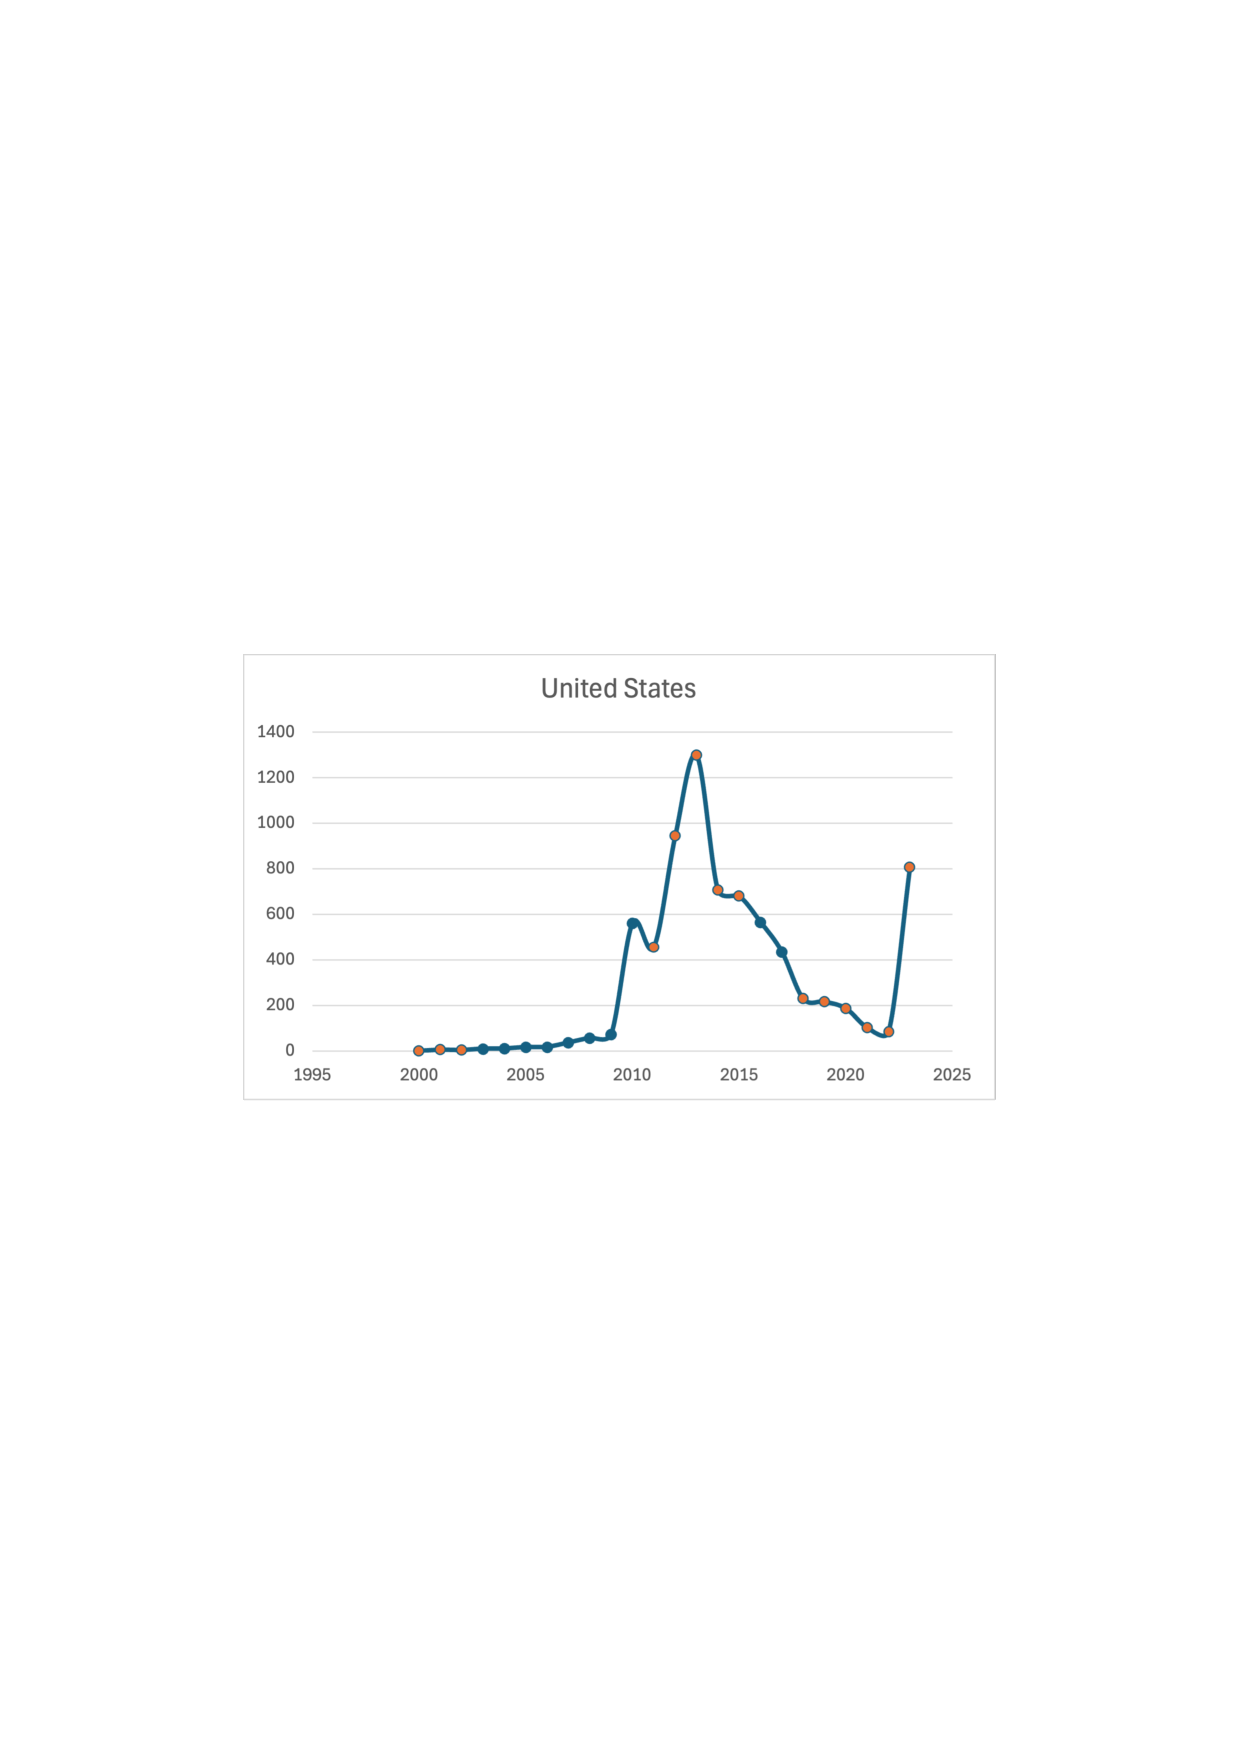
\includegraphics[width=0.45\linewidth]{../rsrc/policies/(T1)US_policy}
        }\hfill
        \subfloat[Japan (T2)]{
            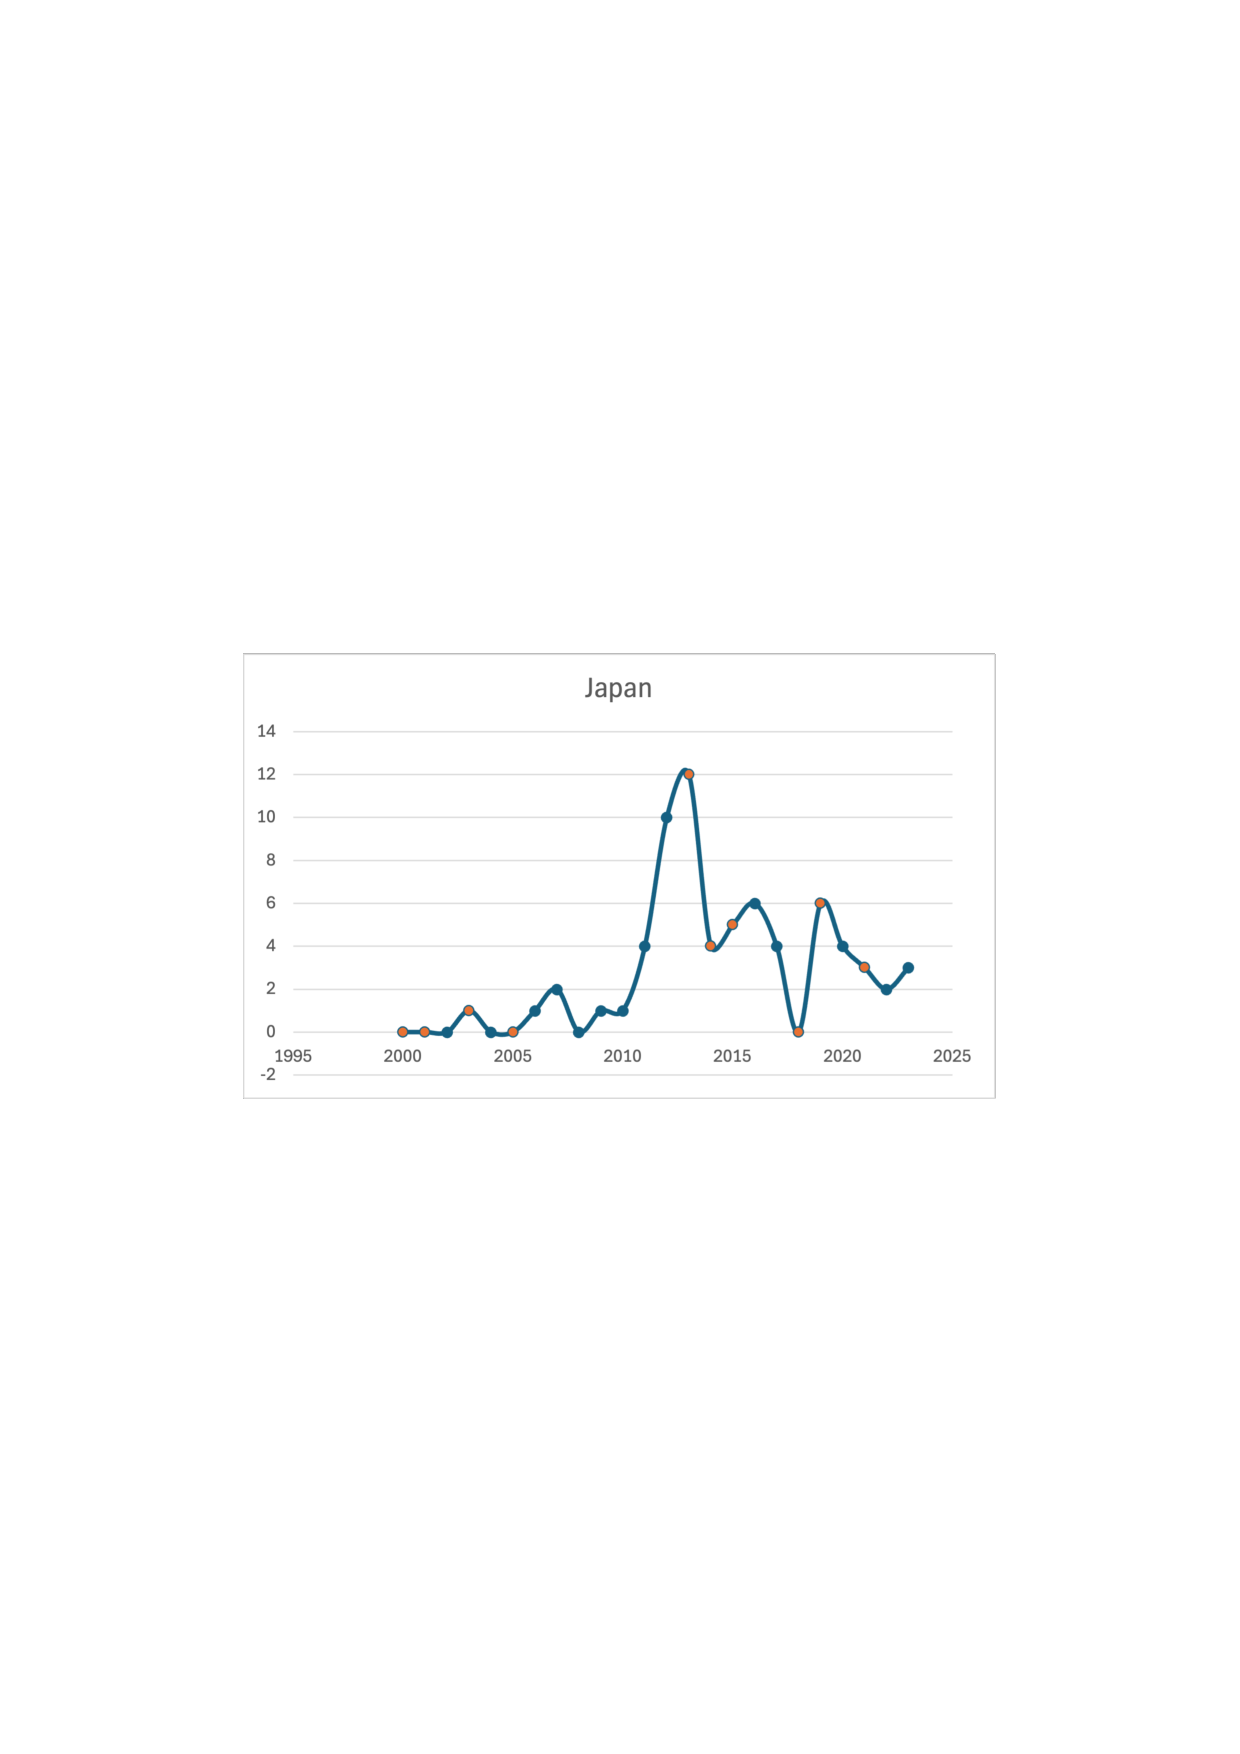
\includegraphics[width=0.45\linewidth]{../rsrc/policies/(T2)Japan_policy}
        }\\
        \subfloat[China (T3)]{
            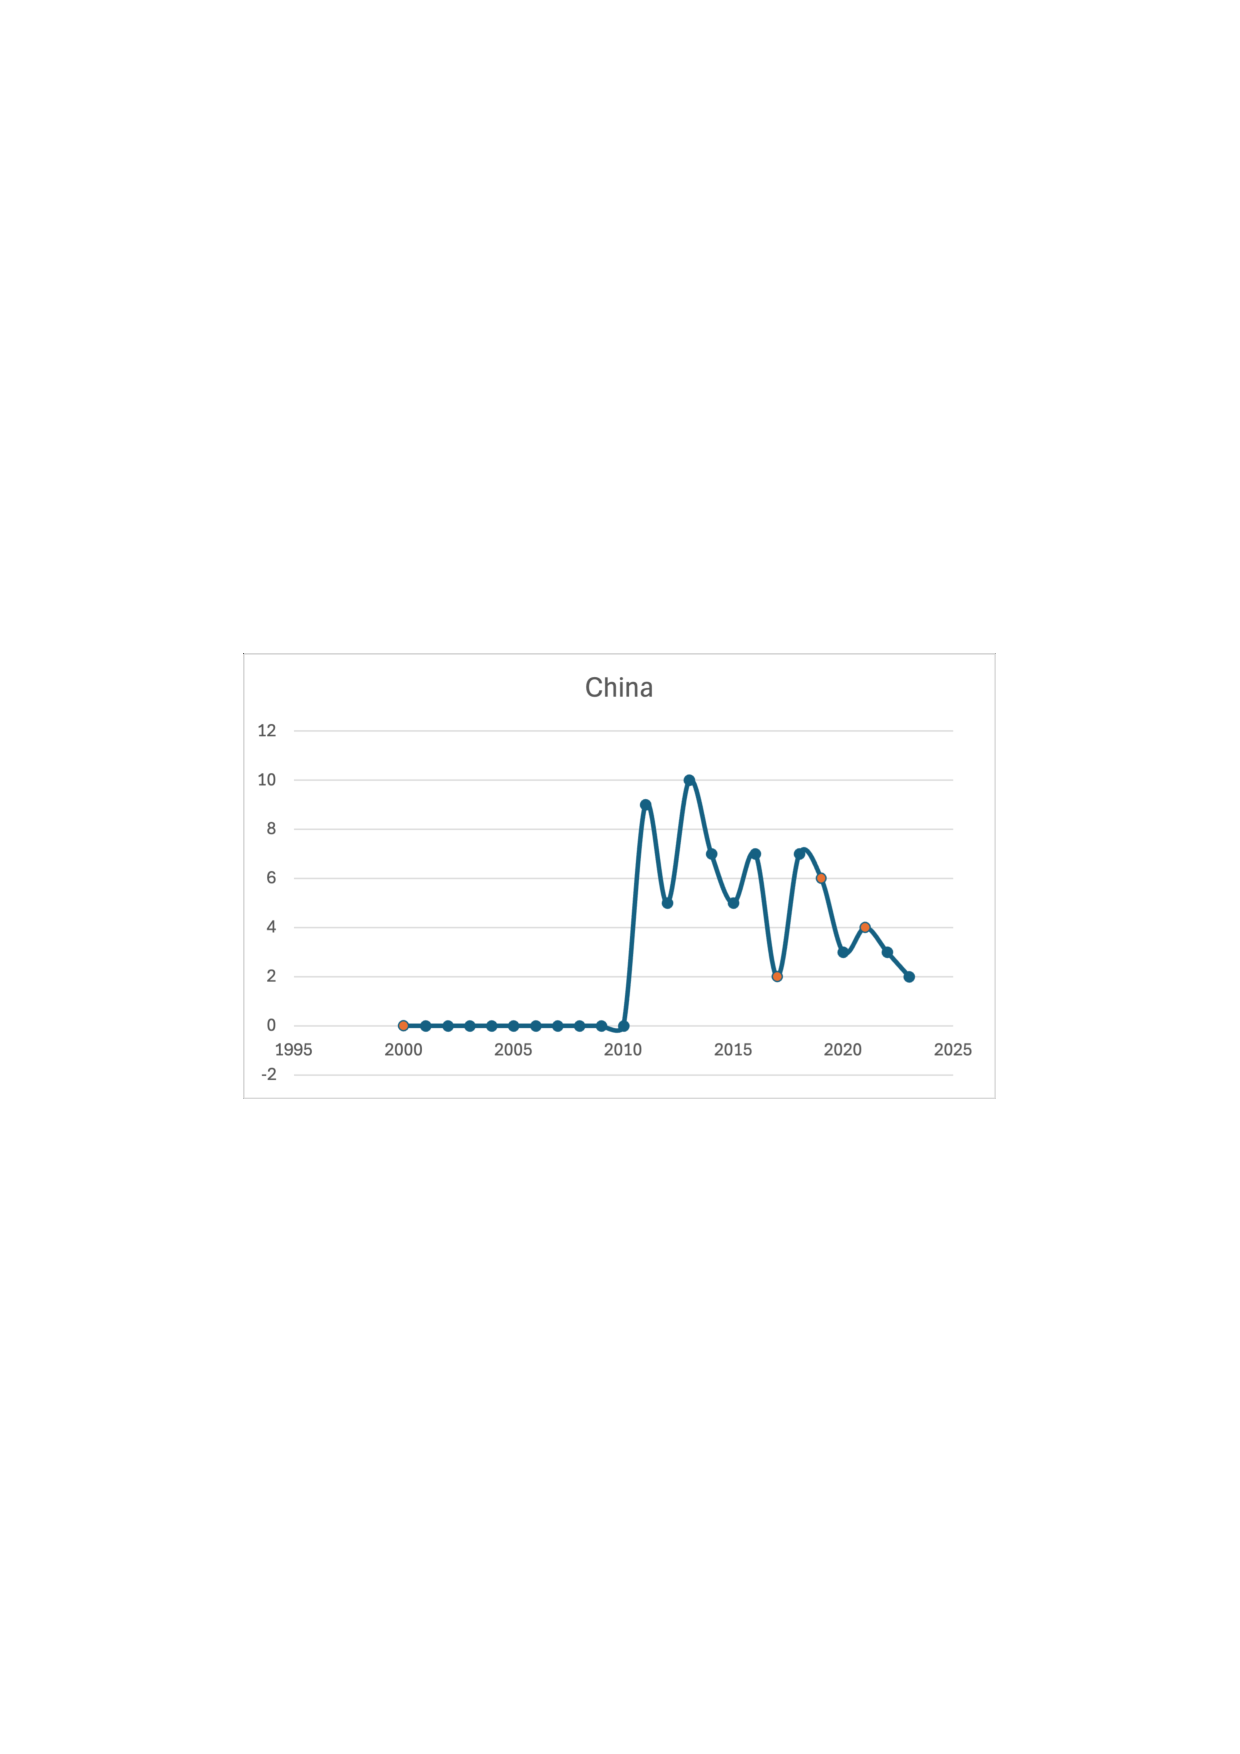
\includegraphics[width=0.3\linewidth]{../rsrc/policies/(T3)China_policy}
        }\hfill
        \subfloat[Costa Rica (T4)]{
            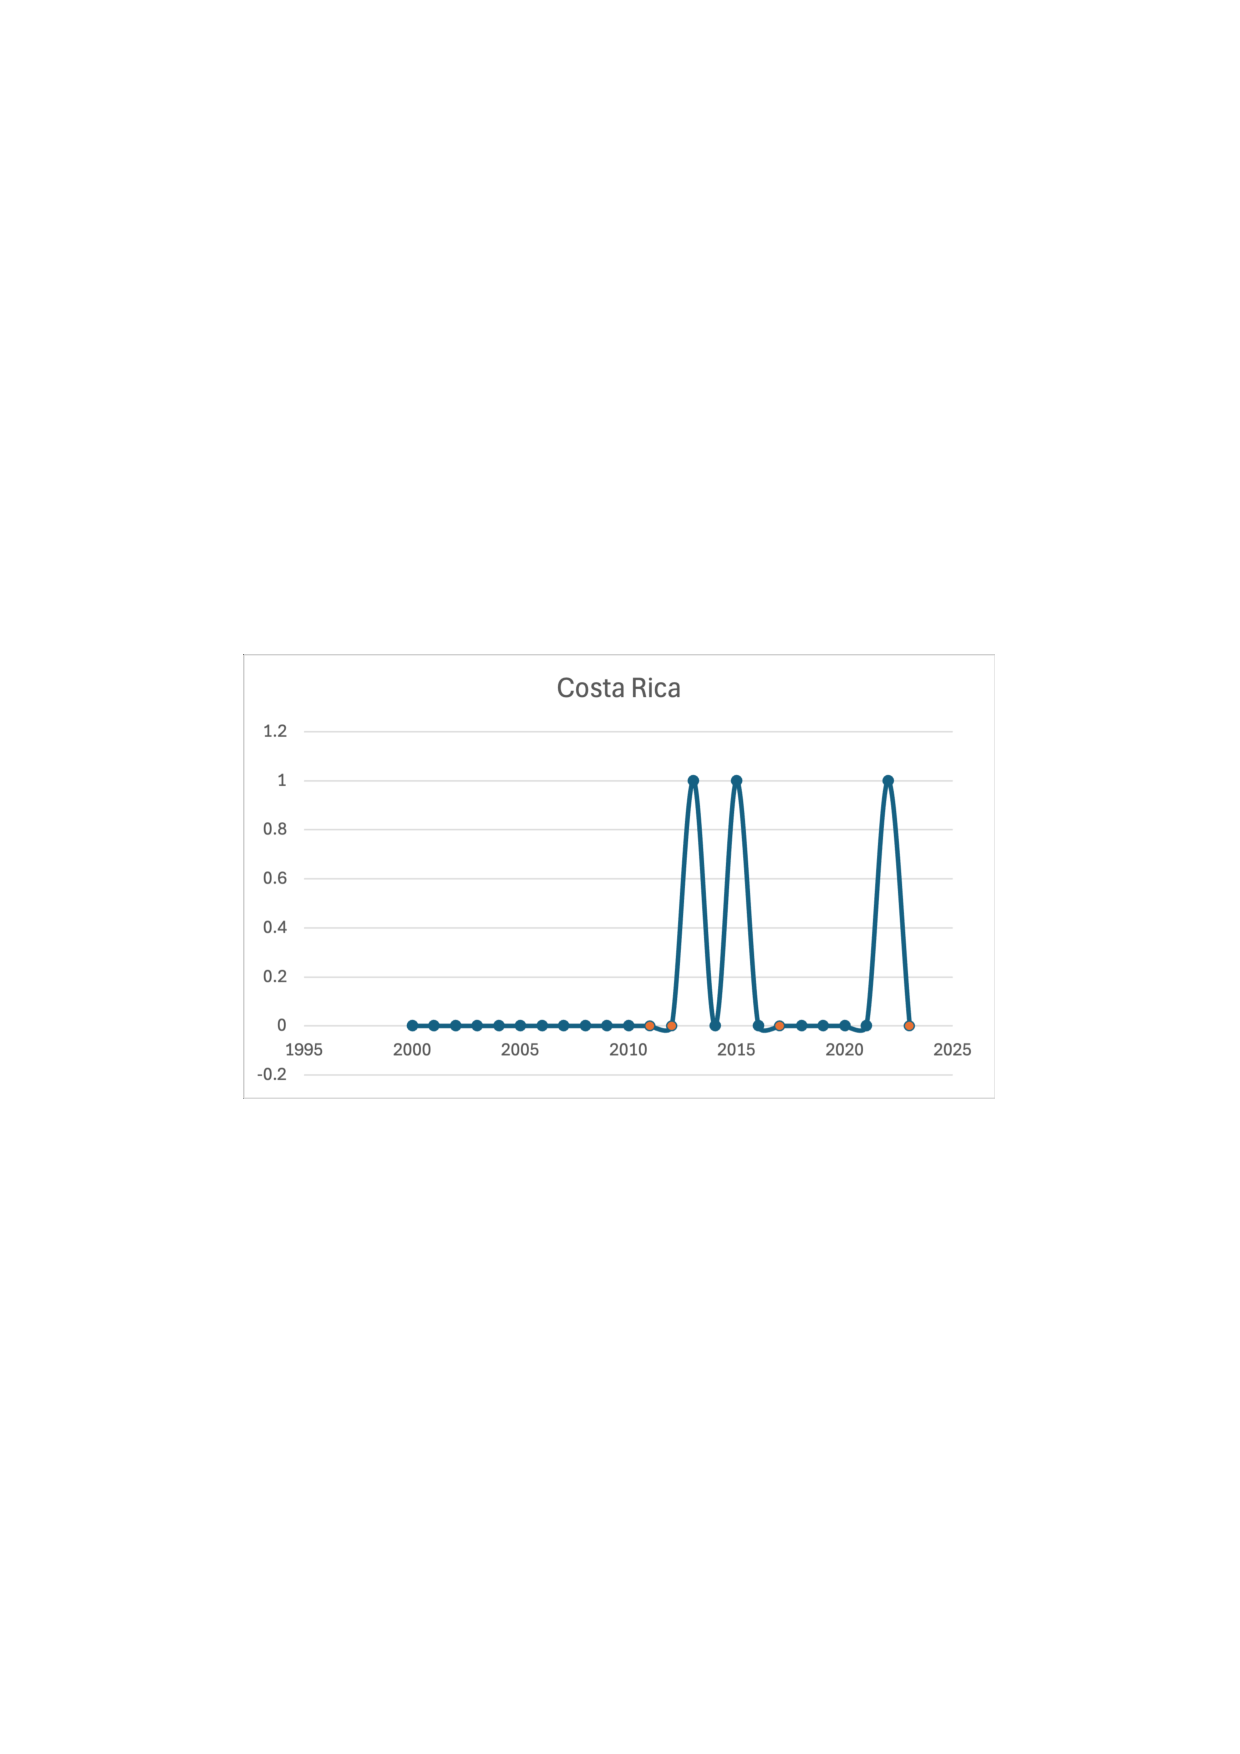
\includegraphics[width=0.3\linewidth]{../rsrc/policies/(T4)Costa_Rica_policy}
        }\hfill
        \subfloat[Namibia (T5)]{
            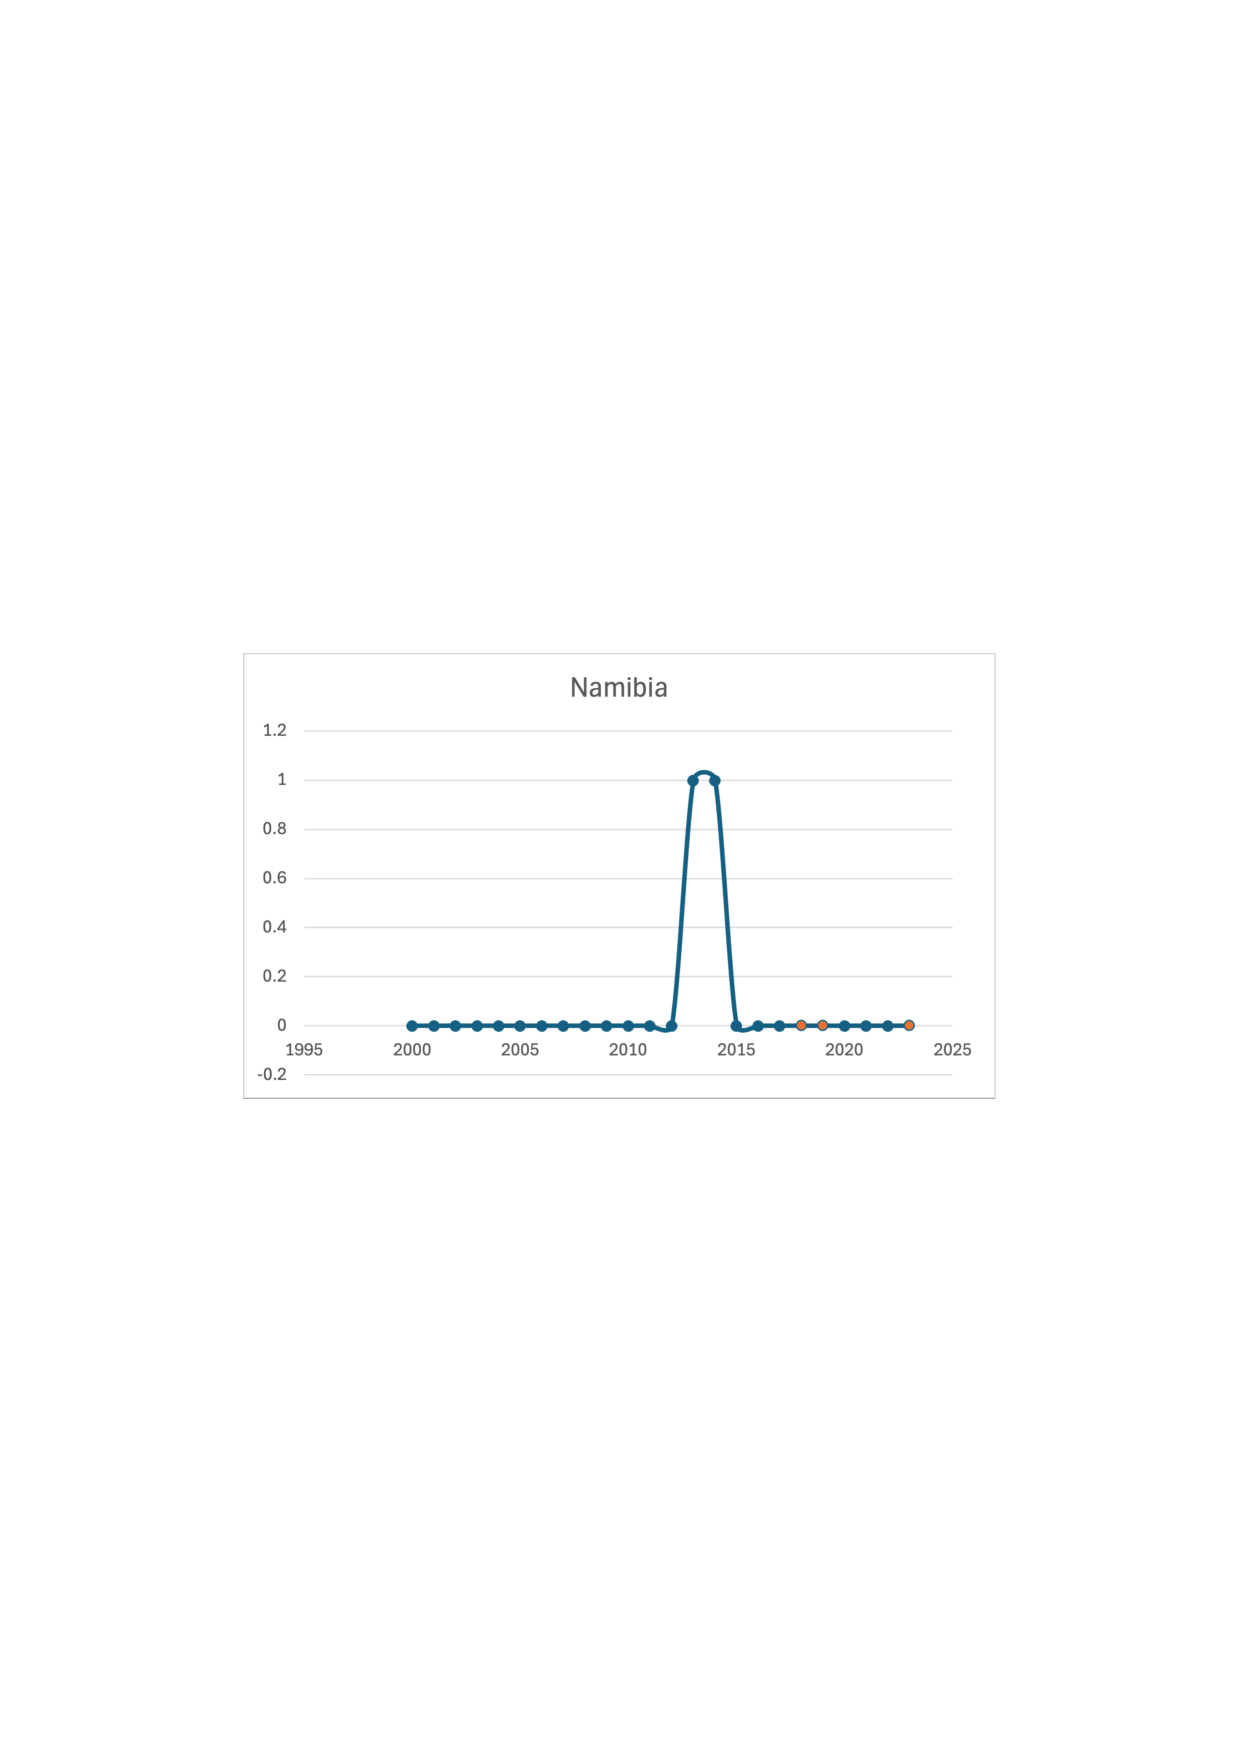
\includegraphics[width=0.3\linewidth]{../rsrc/policies/(T5)Namibia_policy}
        }\\
        \caption{Representative countries}\label{fig:representative-policy}
    \end{figure}

\subsubsection*{Categorizing Policies Based on Effectiveness} %4.1.3
    From the line graphs, we categorize the enacted policies into three sets
    based on the average cybercrime metrics in the years following their implementation compared to the year of enactment.
    Drawing inspiration from fuzzy set theory,
    we assign a value of \(1\) to policies that are effective,
    \(-1\) to those with the opposite effect,
    and values between \(-1\) and \(1\) to policies with varying degrees of impact.
    Specifically:

    \begin{itemize}
        \item \textbf{Effective Policies \( (Value \to 1) \):}
            These are policies where the average cybercrime metrics in the years following enactment
            are lower than those in the year of enactment.
            Examples include:
            \begin{itemize}
                \item National Institute of Standards and Technology (NIST) Cybersecurity Framework (2014)
                \item National Cyber Security Centre (NCSC) Establishment (2016)
                \item Investigatory Powers Act (2016)
                \item Cybersecurity Strategy (2013)
                \item Telecommunications Business Act Amendments (2019)
                \item Cryptography Law of the People’s Republic of China (2019)
            \end{itemize}

        \item \textbf{Counterproductive Policies \( (Value \to -1) \):}
            These are policies where the average cybercrime metrics in the years following enactment
            are higher than those in the year of enactment.
            Examples include:
            \begin{itemize}
                \item Cyber Incident Reporting for Critical Infrastructure Act (CIRCIA) (2022)
                \item Quantum Computing Cybersecurity Preparedness Act (2022)
                \item Strengthening American Cybersecurity Act (2022)
                \item CHIPS and Science Act (2022)
                \item Cybersecurity Strategy (2018)
                \item Cybersecurity Law of the People’s Republic of China (2017)
            \end{itemize}

        \item \textbf{Neutral or Mixed-Impact Policies (Values around 0):}
            These are policies where
            the average cybercrime metrics show no significant change, or the impact is ambiguous.
            Representative examples include:
            \begin{itemize}
                \item Policy A
                \item Policy B
                \item Policy C
                \item (Additional policies to be listed)
            \end{itemize}
    \end{itemize}

    This categorization provides a structured framework for analyzing the effectiveness of cybersecurity policies and
    serves as a basis for further investigation into the factors that contribute to their success or failure.

